%%%%%%%%%%%%%%%%%%%%%%%%%%%%%%%%%%%%%%%%%
% Seismica Submission Template
%%%%%%%%%%%%%%%%%%%%%%%%%%%%%%%%%%%%%%%%%

%% Options available: 
%%					anonymous
%%					breakmath
%%					languages
%%					preprint
%%					report

%% anonymous: produces an anonymous PDF for double-blind review. Will NOT print authors information and acknowledgements, but WILL PRINT data availibility section, so be careful!
%% breakmath: for manuscripts with many long formulas, you can specify the breakmath option (loads the package breqn and uses the dmath environment)
%% languages: see below, use to add abstract(s) in additional languages
%% preprint: removes line numbers, switch to two-columns
%% report: if this is a report

% \documentclass[breakmath,report]{seismica}
\documentclass[preprint]{seismica}

% import packages
\usepackage{amssymb, nicefrac, bm, tikz}


\title{Single-seismometer Focal Mechanism and Uncertainty Estimation from Body Waves}
\shorttitle{Single-seismometer Focal Mechanism and Uncertainty Estimation} % used for header, not mandatory

%% If this is a REPORT, select a report type within: 
%\reporttype{Null Results Report} % (null-results/failed experiments)
%\reporttype{Software Report}
%\reporttype{Data Report} %  (e.g., Large Community dataset initiatives, Instrument Deployments, and Field Campaigns)
%\reporttype{Fast Report}

%% Will not be printed if anonymous option ON
\author[1]{Victor Agaba
	% \orcid{0000-0000-0000-0000}
	\thanks{Corresponding author: victoragaba2025@u.northwestern.edu}
}
\author[1]{Suzan van der Lee
	\orcid{0000-0003-1884-1185}
}
\author[2]{Madelyn Sita
	\orcid{0000-0002-7214-7058}
}
\author[3]{Caio Ciardelli}
\author[4]{Paula Babirye}
\affil[1]{Department of Earth and Planetary Sciences, Northwestern University, Evanston, IL, USA}
\affil[2]{Department of Chemistry, University of Virginia, Charlottesville, VS, USA}

%% Author CRediT roles
%% Please use the CRediT roles as defined at https://casrai.org/credit
%% Use as many roles as necessary; there is no requirement to use all 14 roles
\credit{Conceptualization}{SL, MS.}
\credit{Methodology}{VA, SL.}
\credit{Software}{VA.}
%\credit{Validation}{people}
\credit{Formal Analysis}{VA, SL.}
%\credit{Investigation}{people}
%\credit{Resources}{people}
\credit{Writing - Original draft}{VA, SL.}
%\credit{Writing - Review \& Editing}{people}
\credit{Visualization}{VA, SL.}
\credit{Supervision}{SL.}
%\credit{Project administration}{people}
%\credit{Funding acquisition}{people}


%%%%%%%%%%%%%%%%%%%%%%%%%%%%%%%%%%%%%%%%%
%% Abstracts in other languages
%%%%%%%%%%%%%%%%%%%%%%%%%%%%%%%%%%%%%%%%%
%% If your article includes abstracts in other languages, uncomment the lines below and fill in
%%      the appropriate sections. You will need to use the [languages] option at the top,
%%      and will need to use lualatex instead of pdflatex to compile the document.
%% We will use luatex, polyglossia and fontspec for the compilation of the accepted version. 
%% Feel free to use any polyglossia command.
%\setotherlanguages{french,thai}  % replace with your language(s), per polyglossia
%% if an additional font is needed for the abstract, load it with:
%\newfontfamily\thaifont[Script=Thai]{Noto Serif Thai}

%% If you are using Arabic, do not include it in \setotherlanguages{} as it is not supported 
%% by polyglossia. Instead, with the [languages] option at the top, you can use these commands
%% within the text:
%%\begin{Arabic} and \end{Arabic} around paragraphs in Arabic
%%\n{} to wrap any digits within Arabic text that should read left-to-right
%%\textarabic{} for Arabic text embedded in a left-to-right paragraph

%% also see https://www.overleaf.com/latex/examples/how-to-write-multilingual-text-with-different-scripts-in-latex/wfdxqhcyyjxz for reference
%%%%%%%%%%%%%%%%%%%%%%%%%%%%%%%%%%%%%%%%%

%%%%%%%%%%%%%%%%%%%%%%%%%%%%%%%%%%%%%%%%%
%% Several abstracts
%%%%%%%%%%%%%%%%%%%%%%%%%%%%%%%%%%%%%%%%%
%% the command \makeseistitle does not allow page breaks in preprint mode. If you have
%%		many abstracts, you can use the command \addsummaries. It will induce a pagebreak.

\begin{document}
    \makeseistitle{
        \begin{summary}{Abstract}
            Work on later, 200-word max.
        \end{summary}
        \begin{summary}{Non-technical summary}
            Work on later, shorter than abstract.
        \end{summary}
    }
	
    %%%% In preprint mode, in case you have too many abstracts and need a page break, use this:
    %\addsummaries{
        %	\begin{french}
            %	\begin{summary}{Résumé} 
                %	The text goes here. Again, no longer than 200 words.
                %	\end{summary}
            %	\end{french}
        %	\begin{summary}{Non-technical summary}
            %	The text goes here. Again, no longer than 200 words.
            %	\end{summary}
        %}  %% don't forget this one!
	
\section{Introduction} \label{sec:introduction}

    [Suzan] Insert words here...\\
    Writing tip: maximize information content of words

\section{Cosine similarity misfit criterion} \label{sec:misfit}

  \subsection{Background}
    When a quake event happens, a single seismometer reads $P$, $SV$ and $SH$ body waves through
    which the respective amplitudes $A^P$, $A^{SV}$ and $A^{SH}$ along with their noise levels
    $\sigma_P$, $\sigma_{SV}$ and $\sigma_{SH}$ (representing standard deviation of an assumed normal
    distribution centered at the amplitude value) can be extracted.
    Given a ray path's azimuth $\phi$ and take-off angles $i$, $j$ of $P$ and $S$ waves respectively,
    we model the amplitudes as functions of the source mechanism's fault strike $\psi$, fault dip
    $\delta$ and slip rake $\lambda$, further accounting for the $P$- and $S$-velocities $\alpha_h$,
    $\beta_h$ at source depth $h$ \citep{AkiRichards1980}. The expressions are:

    \begin{align} \label{eq:1}
      \nonumber &A^P \sim \left( s_R(3\cos^2(i) - 1) - q_R\sin(2i) - p_R\sin^2(i)\right)/\alpha_h^3\\
      \nonumber &A^{SV} \sim \left( 1.5 s_R\sin(2j) + q_R\cos(2j) + 0.5 p_R\sin(2j) \right)/\beta_h^3\\
      &A^{SH} \sim \left( q_L\cos(j) + p_L\sin(j) \right)/\beta_h^3
    \end{align}

    where

    \begin{align} \label{eq:2}
      \nonumber s_R &= 0.5 \sin(\lambda) \sin(2\delta)\\
      \nonumber q_R &= \sin(\lambda) \cos(2\delta) \sin(\psi_r) + \cos(\lambda) \cos(\delta) \cos(\psi_r)\\
      \nonumber p_R &= \cos(\lambda) \sin(\delta) \sin(2\psi_r) - 0.5\sin(\lambda) \sin(2\delta) \cos(2\psi_r)\\
      \nonumber p_L &= 0.5\sin(\lambda) \sin(2\delta) \sin(2\psi_r) + \cos(\lambda) \sin(\delta) \cos(2\psi_r)\\
      q_L &= -\cos(\lambda) \cos(\delta) \sin(\psi_r) + \sin(\lambda) \cos(2\delta) \cos(\psi_r)
    \end{align}

    Our goal is two-fold:
    \begin{enumerate}
      \item [i)]
        Find estimates $\widehat{\psi}, \widehat{\delta}, \widehat{\lambda}$ for the strike, dip
        and rake that \textit{best} describe the collected data.

      \item [ii)]
        Estimate the joint noise distribution of fault parameters to more accurately constrain the
        set of \textit{acceptable} estimates for the source mechanism.
        
    \end{enumerate}

    We thus need a metric against which to evaluate what the best and acceptable estimates are. The
    misfit function used by \citet{sita_potential_2022} is defined as the angle between the vector of
    observed amplitudes and that produced from a forward simulation of synthetic parameters.
    In this paper, we shall use a misfit $\Phi$ of negative cosine similarity between the two vectors
    which has a 1-to-1 correspondence with angle:

    \begin{align} \label{eq:3}
      \Phi(\bm{p}) = \frac{-\bm{A}_o^\top\bm{A}_s}{\|\bm{A}_o\|\|\bm{A}_s\|}
    \end{align}

    where $\bm{A}_o = (A_o^P, A_o^{SV}, A_o^{SH})^\top$ are observed amplitudes, $\bm{A}_s =
    (A_s^P, A_s^{SV}, A_s^{SH})^\top$ are synthetic amplitudes, and
    $\bm{p} = (\psi, \delta, \lambda)^\top$ are the underlying parameters.

  \subsection{Justification}
    We are interested in situations where absolute amplitudes are either unknown or unnecessary, for
    instance if using data collected from NASA's Insight mission \citep{sita_potential_2022}.
    In this case, we cannot know the absolute velocities because they depend on an understanding of
    Mars' interior that is good enough to build a reliable velocity model. Alternative misfit
    functions can account for the relative amplitudes, such as in equations \ref{eq:4} and
    \ref{eq:5}:

    \begin{align} \label{eq:4}
      \Phi(\bm{p}) = \sqrt{\left( \Delta \frac{A^{P}}{A^{SV}}\right)^2 + \left( \Delta \frac{A^{SV}}{A^{SH}}\right)^2}
    \end{align}

    \begin{align} \label{eq:5}
      \Phi(\bm{p}) = \sqrt{\log^2 \left( \Delta \frac{A^P}{A^{SV}} \right) + \log^2 \left( \Delta \frac{A^{SV}}{A^{SH}} \right)}
    \end{align}

    First, we note that using cosine similarity is more numerically stable in cases where one of the
    observed or synthetic amplitudes is close to zero since the norm of the associated vector in
    equation \ref{eq:3} may still be large enough to make division feasible.

    Secondly, we have chosen cosine similarity over angle because it involves one less operation,
    which is more computationally efficient and easier to differentiate for directed search
    algorithms (see Section \ref{sec:algorithms}). The Gaussian function in equation \ref{eq:6} is
    similarly easy to differentiate, but it does not account for relative amplitudes so it would
    exclude otherwise acceptable solutions.

    \begin{align} \label{eq:6}
      &\Phi(\bm{p}) \sim |\Sigma|^{-1/2} \exp \left( - \frac{1}{2} (\bm{A} - \bm{A}_o)^\top \bm{\Sigma}^{-1} (\bm{A} - \bm{A}_o) \right)
    \end{align}

  \subsection{Tolerance derivation}
    Given vectors $\bm{A}_s$ and $\bm{A}_o$, we would like to know the largest cosine
    similarity for which $\bm{A}_s$ is considered an acceptable fit with respect to the recorded amplitudes
    while accounting for the asymmetry of error levels for different amplitudes. Visualized in 3D
    space, we have a confidence ellipsoid centered at $\bm{A}_o$ (equation \ref{eq:7}) such that
    acceptable fits are vectors which fall inside the elliptical cone tangent to it with vertex at the
    origin.
    \begin{align} \label{eq:7}
      E(\bm{p}) = (\bm{A} - \bm{A}_o)^\top \tilde{\bm{\Sigma}}^{-1} (\bm{A} - \bm{A}_o)  = 1
    \end{align}
    
    \noindent where $\bm{A} = (A^P, A^{SV}, A^{SH})^\top$ is arbitrary
    and $\tilde{\bm{\Sigma}} = \text{diag}(\sigma_P^2, \sigma_{SV}^2, \sigma_{SH}^2)/\chi^2_{2,\alpha}$ for some $\alpha \in (0,1)$. The elliptical
    cone intersects with the ellipsoid at every boundary point for which
    \begin{align} \label{eq:8}
      (\nabla_{\bm{A}} E)^\top \bm{A} = 2(\bm{A} - \bm{A}_o)^\top \tilde{\bm{\Sigma}}^{-1} \bm{A} = 0
    \end{align}
    
    Combining equations \ref{eq:7} and \ref{eq:8} gives the plane containing every point of 
    tangency:
    \begin{align} \label{eq:9}
      \frac{1}{2} (\nabla_{\bm{A}} E)^\top \bm{A} - f(\bm{A}) = 
              \bm{A}_o^\top \tilde{\bm{\Sigma}}^{-1} (\bm{A} - \bm{A}_o)  = -1
    \end{align}

    To account for asymmetry, we recognize that the orientation of $\bm{A}_s$ relative to $\bm{A}_o$
    has an effect on the tolerance because the associated "thickness" of the ellipsoid changes.
    This information is captured by the plane containing vectors $\bm{A}_o$ and $\bm{A}_s$:
    \begin{align} \label{eq:10}
      (\bm{A}_s \times \bm{A}_o)^\top \bm{A} = 0
    \end{align}

    To find the constrained points of tangency, we can intersect the original ellipsoid with planes
    \ref{eq:9} and \ref{eq:10}. The line of intersection is such that
    \begin{align} \label{eq:11}
      \bm{A}(t) = (1 - \nicefrac{1}{c_1}) \bm{A}_o + t\bm{D}
    \end{align}

    \noindent where $c_1$ (equation \ref{eq:12}) is a location parameter projecting $\bm{A}_o$ onto plane \ref{eq:9}
    and $\bm{D}$ (equation \ref{eq:13}) is the direction perpendicular to planes \ref{eq:9} and \ref{eq:10}. 

    \begin{align} \label{eq:12}
      \nonumber \bm{A}_o^\top \tilde{\bm{\Sigma}}^{-1} ((1 - \nicefrac{1}{c_1})\bm{A}_o - \bm{A}_o)  = -1\\
      \Rightarrow c_1 = \bm{A}_o^\top \tilde{\bm{\Sigma}}^{-1} \bm{A}_o = \|\bm{A}_o\|_{\tilde{\bm{\Sigma}}^{-1}}^2
    \end{align}
    \begin{align} \label{eq:13}
      \nonumber\bm{D} &= (\bm{A}_o^\top \tilde{\bm{\Sigma}}^{-1})^\top \times (\bm{A}_s \times \bm{A}_o)\\
        &= c_1\bm{A}_s - c_2\bm{A}_o
    \end{align}

    \noindent where $c_2 = \bm{A}_o^\top \tilde{\bm{\Sigma}}^{-1} \bm{A}_s = \langle\bm{A}_o^\top, \bm{A}_s\rangle_{\tilde{\bm{\Sigma}}^{-1}}$.

    Combining equations \ref{eq:7} and \ref{eq:11} produces a quadratic parameterized by the scalar $t$,
    from which we can obtain a quadratic equation for the points of tangency:

    \begin{align} \label{eq:14}
      \nonumber (t\bm{D} - \nicefrac{1}{c_1}\bm{A}_o)^\top \tilde{\bm{\Sigma}}^{-1} (t\bm{D} - \nicefrac{1}{c_1}\bm{A}_o)  = 1\\
      ({\bm{D}^\top \tilde{\bm{\Sigma}}^{-1} \bm{D}})t^2 - 
          \nicefrac{2}{c_1}(\bm{A}_o^\top \tilde{\bm{\Sigma}}^{-1} \bm{D})t + (\nicefrac{1}{c_1} - 1) = 0
    \end{align}

    Denote $c_3 = \bm{A}_s^\top \tilde{\bm{\Sigma}}^{-1} \bm{A}_s = \|\bm{A}_s\|_{\tilde{\bm{\Sigma}}^{-1}}^2$. Then by
    substitution we have
    ${\bm{D}^\top \tilde{\bm{\Sigma}}^{-1} \bm{D}} = c_1(c_1c_3 - c_2^2)$ and ${\bm{A}_o^\top \tilde{\bm{\Sigma}}^{-1} \bm{D}} = 0$.
    Solving then yields the necessary points (denoted $\bm{A}_b$) as
    \begin{align} \label{eq:15}
      \bm{A}_b = \left(1 - \frac{1}{c_1}\right)\bm{A}_o \pm
        \left(\frac{1}{c_1} \sqrt{\frac{c_1 - 1}{c_1c_3 - c_2^2}}\right)(c_1\bm{A}_s - c_2\bm{A}_o)
    \end{align}

    Equation \ref{eq:15} shows that for the points to be well-defined, the following conditions
    must hold relative to the inner-product space defined by $\tilde{\bm{\Sigma}}^{-1}$:
    
    \begin{itemize}
      \item Strict Cauchy-Schwarz inequality: $c_1c_3 > c_2^2$. This also implies that
        $\tilde{\bm{\Sigma}} \succ 0$ and $\bm{A}_s \nparallel \bm{A}_o$. Practically, it means that all
        uncertainties are necessary and inversion methods that depend on forward simulation should
        treat parallelism as an edge case.
      \item Confidence ellipsoid cannot contain origin: $c_1 \geq 1$. Practically, we should expect
      errors to be a small fraction of observed amplitudes.
    \end{itemize}

    Thus, given 2 nonparallel vectors $\bm{A}_o$ and $\bm{A}_s$ and positive definite covariance
    matrix $\tilde{\bm{\Sigma}}$, we accept the simulation if $\hat{\bm{A}}_o^\top \hat{\bm{A}_s} \geq \text{tol} 
    = \min_b \hat{\bm{A}}_o^\top \hat{\bm{A}_b}$. The condition, more formally, is
    \begin{align} \label{eq:16}
      \max_b \hat{\bm{A}}_o^\top (\hat{\bm{A}}_b - \hat{\bm{A}}_s) \leq 0
    \end{align}

    \noindent where $\hat{\bm{A}}_o$, $\hat{\bm{A}}_s$ and $\hat{\bm{A}}_b$ are unit vectors.


\section{Search Methods} \label{sec:algorithms}
  
  \subsection{Misfit gradient}
    The vector $\bm{A} = (A^P, A^{SV}, A^{SH})^\top$ can be treated as a continuously differentiable 
    nonlinear function of parameters $\bm{p} = (\psi, \delta, \lambda)^\top$, defined by equation 
    \ref{eq:1}. We can thus apply directed search methods to minimize the following cost function:
    \begin{align} \label{eq:17}
      \Phi(\bm{p}) = -\hat{\bm{A}}_o^\top \hat{\bm{A}}
    \end{align}

    To calculate the gradient, first note that $\bm{A}$ is a linear combination of nonlinear functions
    of $\bm{p}$ (equation \ref{eq:2}).



    \begin{figure}[ht!]
      \centering
      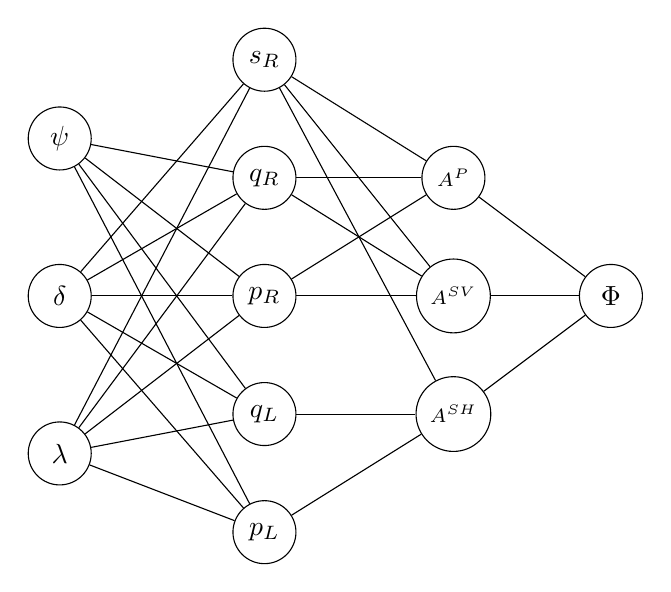
\begin{tikzpicture}[every node/.style={circle, draw, minimum size=.8cm}]
        \node (P1) at (0,2) {$\psi$};
        \node (P2) at (0,0) {$\delta$};
        \node (P3) at (0,-2) {$\lambda$};
        
        \node (H1) at (2.6,3) {$s_R$};
        \node (H2) at (2.6,1.5) {$q_R$};
        \node (H3) at (2.6,0) {$p_R$};
        \node (H4) at (2.6,-1.5) {$q_L$};
        \node (H5) at (2.6,-3) {$p_L$};
        
        \node (A1) at (5,1.5) {\scriptsize $A^P$};
        \node (A2) at (5,0) {\scriptsize $A^{SV}$};
        \node (A3) at (5,-1.5) {\scriptsize $A^{SH}$};
        
        \node (M) at (7,0) {$\Phi$};
        
        \foreach \p in {2,3}
          \foreach \h in {1,2,3,4,5}
            \draw (P\p) -- (H\h);
        
        % \foreach \h in {1,2,3,4,5}
        %   \foreach \a in {1,2,3}
        %     \draw[dashed] (H\h) -- (A\a);
        
        \foreach \a in {1,2,3}
          \draw (A\a) -- (M);
  
        % \draw[dashed] (P1) -- (H1);
        \draw (P1) -- (H2);
        \draw (P1) -- (H3);
        \draw (P1) -- (H4);
        \draw (P1) -- (H5);
  
        \draw (H1) -- (A3);
        \draw (H1) -- (A1);
        \draw (H1) -- (A2);
        \draw (H2) -- (A1);
        \draw (H2) -- (A2);
        \draw (H3) -- (A1);
        \draw (H3) -- (A2);
        \draw (H4) -- (A3);
        \draw (H5) -- (A3);
      \end{tikzpicture}
      \caption{Computational graph of forward model (edges are non-zero partial derivatives).}
      \label{fig:1}
    \end{figure}

    Define a vector $\bm{\eta} = (s_R, q_R, p_R, q_L, p_L)^\top$. Then we can encode
    the misfit as
    \begin{align} \label{eq:18}
      \Phi(\bm{p}) = \Phi(\bm{A}(\bm{\eta}(\bm{p})))
    \end{align}

    \noindent This composition is visualized as a computational graph in figure \ref{fig:1}.
    Each stage of the composition has an associated Jacobian, which we can demonstrate layer by layer:
    
    i) From $\bm{p}$ to $\bm{\eta}$, we can use equation \ref{eq:2} to define the Jacobian
    as follows:
    \begin{align*}
      &a = \sin(\lambda)\;\;\;\;\;\;\;\;\;\;\;\;\; b = \cos(2\delta)\;\;\;\;\;\;\;\;\;\;\; c = \cos(\lambda)\\
      &d = \sin(2\delta)\;\;\;\;\;\;\;\;\;\;\;\; e = \sin(\delta)\;\;\;\;\;\;\;\;\;\;\;\; f = \cos(\delta)\\
      &g = \sin(\psi - \phi)\;\;\;\;\;\; h = \cos(\psi - \phi)\;\;\;\;\; p = cos(2(\psi - \phi))\\
      &q = \sin(2(\psi - \phi))
    \end{align*}
    \begin{align} \label{eq:19}
      \nonumber&\bm{J_p}(\bm{\eta}) = \\
      &\begin{bmatrix}
        0         &ab         &0.5cd\\
        abh-cfg   &-2adg-ceh  &cbg-afh\\
        2cep+adq  &cfq-abp    &-aeq-0.5cdp\\
        -cfh-abg  &ceg-2adh   &afg+cbh\\
        adp-2ceq  &abq+cfp    &0.5cdq-aep
      \end{bmatrix}
    \end{align}

    ii) From $\bm{\eta}$ to $A$, we have a linear transformation whose Jacobian is the matrix
    of coefficients from equation \ref{eq:1}:
    \begin{align} \label{eq:20}
      \nonumber&\bm{J_\eta}(\bm{A}) = \\
      &\begin{bmatrix}
        \frac{3\cos^2(i)-1}{\alpha_h^3}    &\frac{-\sin(2i)}{\alpha_h^3}    &\frac{-sin^2(i)}{\alpha_h^3}   &0    &0\\
        \frac{1.5\sin(2j)}{\beta_h^3}      &\frac{\cos(2j)}{\beta_h^3}      &\frac{0.5\sin(2j)}{\beta_h^3}  &0    &0\\
        0         &0           &0        &\frac{\cos(j)}{\beta_h^3}       &\frac{\sin(j)}{\beta_h^3}
      \end{bmatrix}
    \end{align}

    iii) From $\bm{A}$ to $\Phi$, we have a scalar function whose Jacobian is the gradient
    transposed.
    \begin{align} \label{eq:21}
      \nonumber\nabla_{\bm{A}}\Phi &= \frac{\|\bm{A}\|\nabla_{\bm{A}}(-\hat{\bm{A}}_o^\top\bm{A}) + 
      \hat{\bm{A}}_o^\top \bm{A} \nabla_{\bm{A}}(\|\bm{A}\|)}{\|\bm{A}\|^2}\\
            &= \frac{1}{\|\bm{A}\|}(\Phi\hat{\bm{A}} - \hat{\bm{A}}_o)
    \end{align}

    Combining \ref{eq:19}, \ref{eq:20} and \ref{eq:21} gives the overall gradient:
    \begin{align} \label{eq:22}
      \nabla_{\bm{p}}\Phi = \bm{J_p}(\bm{\eta})^\top \bm{J_\eta}(\bm{A})^\top \nabla_{\bm{A}}\Phi
    \end{align}

  \subsection{Optimization algorithms}
    Something about gradient-based methods. Try different algorithms, they may produce
    interesting results >> IEMS 450-2.

    \noindent \textbf{TODO:} Create one 3D image with the results of gradient descent from random points in space.


\section{Uncertainty Quantification} \label{sec:uncertainty}

    \subsection{Error propagation}
      Say something here, composed Jacobian is important >> Earth 353, IEMS 401.

      \noindent Emphasize the interest in modality.

    \subsection{Monte Carlo methods}
      Place to talk about different seeding stategies and their effect on uncertainty.
      Why hybrid search was used, why systematic over random.
    
    \subsection{Kagan angle}
      An alternative way of quantifying model deviations.


\section{Testing} \label{sec:example}

    \subsection{Synthetic data}
      Say something here about the Monte Carlo
    
    \subsection{Earth data}
      From Uganda (Paula)

    \subsection{Mars data}
      From Insight (Suzan/Maddy)

\section{Conclusions} \label{sec:conclusion}

    \subsection{Performance overview}
      Put some words here...

    \subsection{Growth avenues}
      Put some more words here...

%% Will not be printed if anonymous option ON
\begin{acknowledgements}
    [Suzan] Insert words here...
\end{acknowledgements}

\section*{Data and code availability}
Create a new repo with beautiful code, READMEs and everything. One function/algorithm at a time.

\section*{Competing interests}
    The authors have no competing interests.

%% If the article is accepted, a separate bibfile must be uploaded along with the compiled manuscript, source file, and separate figure files.
%% When available, DOI numbers must be provided for all references, including datasets and codes.
\bibliography{references}
   
\end{document}
	
